\documentclass[12pt]{article}
\usepackage[a4paper, total={6in, 9in}]{geometry}
\usepackage{amsmath, amssymb}
\usepackage{graphicx}
\usepackage{enumitem}
\usepackage{fancyvrb}
\usepackage[skip=\medskipamount]{parskip}
\usepackage{pdfpages}
\usepackage{array}
\usepackage{tabularray}
\usepackage{longtable}
\usepackage{tikz}
\setlength{\parindent}{0pt}

\title{\vspace{-1.5cm}UMC-203 Assignment-2}
\author{Aditya Gupta \\
SR No: 22205}
\date{}

\begin{document}
\maketitle

\section{Support Vector Machine}

\subsection{The binary case}
We are given a dataset with 10 different labels. We choose two labels, which turn out to be 5 and 9 according to my SR No. We name them 1 and -1 respectively. Before proceeding, we augment the data with a 1 to account for the bias term. Then we solve the following optimization problems.

\subsubsection{Primal slack linear SVM}
The primal slack linear SVM problem is defined as follows:
\begin{align*}
    \min_{w, b, \xi} \quad &\frac{1}{2}w^Tw + C\sum_{i=1}^{n}\xi_i \\
    \text{subject to} \quad &y_i(w^Tx_i + b) \geq 1 - \xi_i, \quad i = 1, 2, \ldots, n \\
    &\xi_i \geq 0, \quad i = 1, 2, \ldots, n
\end{align*}

The cvxopt library solves the quadratic minimisation problem as:
\begin{align*}
    \min_{x} \quad &\frac{1}{2}x^TPx + q^Tx \\
    \text{subject to} \quad &Gx \leq h \\
    &Ax = b
\end{align*}

To solve this, we first define the variable $x$ as $[w_1, w_2, \dots ,w_{785}, \xi_1, \xi_2, \dots ,\xi_{1000}]^T$. Here $n=1000$ and dimension of $w$ is 785 (784 + 1 due to augmentation).

Since we have no equalities here, $A$ and $b$ are 0. We define the matrices $P, q, G, h$ as follows:
\begin{align*}
    P &= \begin{bmatrix}
        I_{784 \times 784} & 0_{784 \times 1001} \\
        0_{1001 \times 784} & 0_{1001 \times 1001} \\
    \end{bmatrix} \\ \\
    q &= [0_{784}, 0_{1000}]^T \\ \\
\end{align*}

\begin{align*}
    G &= \begin{bmatrix}
        -y_1x_1^T \\ 
        \vdots & -I_{1000 \times 1000} \\ 
        -y_{1000}x_{1000}^T \\
        0_{1000 \times 785} & -I_{1000 \times 1000} \\
    \end{bmatrix} \\ \\
    h &= [-1_{1000}, 0_{1000}]^T
\end{align*}

The accuracies received for different values of $C$ are:
\begin{center}
    \begin{tabular}{|c|c|}
        \hline
        $C$ & Accuracy \\
        \hline
        1 & 97.5 \% \\
        10 & 97.5 \% \\
        100 & 97.5 \% \\
        \hline
    \end{tabular}
\end{center}

\subsubsection{Dual slack linear SVM}
The dual slack linear SVM problem is defined as follows:
\begin{align*}
    \max_{\alpha} \quad &\sum_{i=1}^{n}\alpha_i - \frac{1}{2}\sum_{i=1}^{n}\sum_{j=1}^{n}\alpha_i\alpha_jy_iy_jx_i^Tx_j \\
    \text{subject to} \quad &0 \leq \alpha_i \leq C, \quad i = 1, 2, \ldots, n \\
    &\sum_{i=1}^{n}\alpha_iy_i = 0 \\
    w &= \sum_{i=1}^{n}\alpha_iy_ix_i
\end{align*}

To solve this in cvxopt, we first define the variable $x$ as $[\alpha_1, \alpha_2, \dots ,\alpha_{1000}]^T$. We define the matrices $P, q, G, h, A, b$ as follows:
\begin{align*}
    P &= \begin{bmatrix}
        y_1y_1x_1^Tx_1 & y_1y_2x_1^Tx_2 & \dots & y_1y_{1000}x_1^Tx_{1000} \\
        y_2y_1x_2^Tx_1 & y_2y_2x_2^Tx_2 & \dots & y_2y_{1000}x_2^Tx_{1000} \\
        \vdots & \vdots & \ddots & \vdots \\
        y_{1000}y_1x_{1000}^Tx_1 & y_{1000}y_2x_{1000}^Tx_2 & \dots & y_{1000}y_{1000}x_{1000}^Tx_{1000} \\
    \end{bmatrix} \\ \\
    q &= [-1_{1000}]^T \\ \\
    G &= \begin{bmatrix}
        -I_{1000 \times 1000} \\
        I_{1000 \times 1000}
    \end{bmatrix} \\ \\
\end{align*}
\begin{align*}
    h &= \begin{bmatrix}
        0_{1000} \\
        C_{1000}
    \end{bmatrix} \\ \\
    A &= y^T \\ \\
    b &= [0]
\end{align*}

The accuracies received for different values of $C$ are:
\begin{center}
    \begin{tabular}{|c|c|}
        \hline
        $C$ & Accuracy \\
        \hline
        1 & 65 \% \\
        10 & 65 \% \\
        100 & 65 \% \\
        \hline
    \end{tabular}
\end{center}

The reduced accuracy of the dual can be attributed to the fact that we do not have a good way to get the value of the bias for the dual problem. (the accuracy is higher for some other random SR No values, since the bias term changes for every dataset)

\subsubsection{Kernelized SVM}
The kernelized SVM problem is defined as follows:
\begin{align*}
    \max_{\alpha} \quad &\sum_{i=1}^{n}\alpha_i - \frac{1}{2}\sum_{i=1}^{n}\sum_{j=1}^{n}\alpha_i\alpha_jy_iy_jK(x_i, x_j) \\
    \text{subject to} \quad &0 \leq \alpha_i \leq C, \quad i = 1, 2, \ldots, n \\
    &\sum_{i=1}^{n}\alpha_iy_i = 0
\end{align*}

The accuracies received for different values of $C$ are:
\begin{center}
    \begin{tabular}{|c|c|}
        \hline
        $C$ & Accuracy \\
        \hline
        1 & 50 \% \\
        10 & 50 \% \\
        100 & 50 \% \\
        \hline
    \end{tabular}
\end{center}

\subsubsection{Scikit-learn linear SVM}
The accuracies received for different values of $C$ are:
\begin{center}
    \begin{tabular}{|c|c|}
        \hline
        $C$ & Accuracy \\
        \hline
        1 & 100 \% \\
        10 & 100 \% \\
        100 & 100 \% \\
        \hline
    \end{tabular}
\end{center}


\subsection{Multiclass SVM}
\subsubsection{Classifier}
The multiclass classifier can be given as:
\begin{align*}
    h(x) = \underset{i \in \{1,\dots,k\}}{argmax} \{w_i^Tx\}
\end{align*}

\subsubsection{Lagrangian Dual}
To solve the multiclass Lagrangian, we introduce the Kronecker delta in the primal SVM problem. The primal problem can be given as:
\begin{align*}
    \min_{w_i, \xi_i} \quad &\frac{1}{2}\sum_{k=1}^{K}w_k^Tw_k + C\sum_{i=1}^{n}\xi_i \\
    \text{subject to} \quad &w_{y_i}^Tx_i - w_{k}^Tx_i \geq 1 - \xi_i - \delta_{y_i,k} \quad (x_i,y_i) \in D \\
    &k = 1, 2, \ldots, K
\end{align*}

The Lagrangian can then be given as:
\begin{align*}
    L(w_i, \xi_i, \lambda) &= \frac{1}{2}\sum_{k=1}^{K}w_k^Tw_k + C\sum_{i=1}^{n}\xi_i + \sum_{i=1}^{n}\sum_{k=1}^{K}\lambda_{i,k}(1 - \xi_i - \delta_{y_i,k} - w_{y_i}^Tx_i + w_{k}^Tx_i)
\end{align*}

To solve for optimality, we take derivatives with respect to $w_i$ and $\xi_i$ and set them to 0. We get the following equations:
\begin{align*}
    \frac{\partial L}{\partial \xi_i} = 0 &\implies \sum_{k=1}^{K} \lambda_{i,k} = C \\
    \frac{\partial L}{\partial w_k} = 0 &\implies w_k = - \sum_{i=1}^{n}\lambda_{i,k}x_i + \sum_{i=1}^{n} \left(\sum_{k=1}^{K} \lambda_{i,k}\right)x_i 
\end{align*}

We can solve for $w_k$ further to get:
\begin{align*}
    w_k &= - \sum_{i=1}^{n} \lambda_{i,k}x_i + C\sum_{i=1, y_i=k}^{n} x_i \\
    &= - \sum_{i=1}^{n} \lambda_{i,k}x_i + C\sum_{i=1}^{n} \delta_{y_i,k} x_i \\
    &= \sum_{i=1}^{n} (C \delta_{y_i,k} - \lambda_{i,k}) x_i
\end{align*}

Substituting these values back in $L$, we get:
\begin{align*}
    L(\lambda) = - \frac{1}{2} \left[\sum_{i=1}^{n} \sum_{j=1}^{n} x_i^T x_j \sum_{k=1}^{K} (C \delta_{y_i,k} - \lambda_{i,k})(C \delta_{y_j,l} - \lambda_{j,l})\right] - \left(\sum_{i=1}^{n} \sum_{k=1}^{K} \lambda_{i,k} \delta_{y_i,k}\right)
\end{align*}

Define $\alpha_i = C e_i - \lambda_i = (C \delta_{y_i,1} - \lambda_{i,1}, \dots , C \delta_{y_i,K} - \lambda_{i,K})^T$
\begin{align*}
    \therefore L(\lambda) = - \frac{1}{2} \left[\sum_{i=1}^{n} \sum_{j=1}^{n} (x_i^T x_j) (\alpha_i^T \alpha_j)\right] - \sum_{1}^{n} \alpha_i^T e_i
\end{align*}
where $e_i = (0, \dots, 1, \dots, 0)^T$ with 1 at the $i^{th}$ position.

Now the dual optimization problem can be given by:
\begin{align*}
    \min_{\alpha_1, \dots, \alpha_n} \quad &\frac{1}{2} \left[\sum_{i=1}^{n} \sum_{j=1}^{n} (x_i^T x_j) (\alpha_i^T \alpha_j)\right] + \sum_{1}^{n} \alpha_i^T e_i \\
    \text{subject to} \quad &\sum_{k=1}^{K} \alpha_{i,k} = 0 \quad \forall i \in \{1, \dots, n\}\\
    &\alpha_i^k \le 0, \ \text{if} \ y_i \ne k \\
    &\alpha_i^k \le C, \ \text{if} \ y_i = k \\
    &w_k = \sum_{i=1}^{n} \alpha_i^k x_i
\end{align*}


\section{Regression}
\subsection{Linear Regression}
After loading the dataset, I have omitted the first two columns, ie ID and Date. Then the first 80\% of the dataset was used as training data and the remaining 20\% was used as testing data. The labels are the prices of the houses and the features are the remaining columns.

Before applying regression, the data was augmented with a 1 to account for the bias term. The regression was then applied to the training data to obtain $w$ using the following formula:
\begin{align*}
    w_{LR} &= (X^TX)^{-1}X^TY \\
    w_{RR} &= (X^TX + \lambda I)^{-1}X^TY
\end{align*}
where $X$ is the augmented training data and $Y$ is the true labels.

On solving the regression, the MSE was:
\begin{align*}
    MSE_{LR} &= 7 \times 10^{11} \\
    MSE_{RR} &= 2 \times 10^{10}
\end{align*}

Since $w$ is not a 1-D number, we can not directly draw a line with slope $w$ on a 2-D plane. To show the line, we connect all the points predicted by the regression and plot it against the actual values.

The plot for the actual values vs the prediction by the linear regression model is:
\begin{center}
    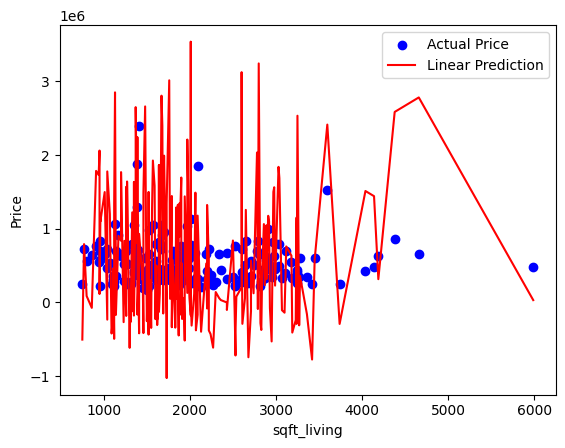
\includegraphics[width=0.8\textwidth]{img/linear.png}
\end{center}

The plot for the actual values vs the prediction by the ridge regression model is:
\begin{center}
    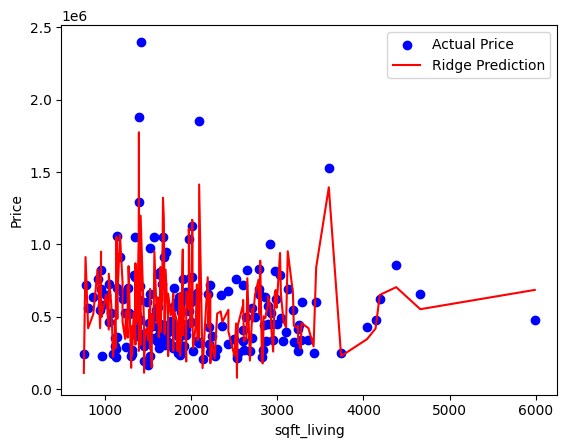
\includegraphics[width=0.8\textwidth]{img/ridge.png}
\end{center}

\subsection{Gaussian Process Regression}
The Gaussian Process Regression was applied to the same dataset with different kernels. The results were as follows:

\begin{center}
    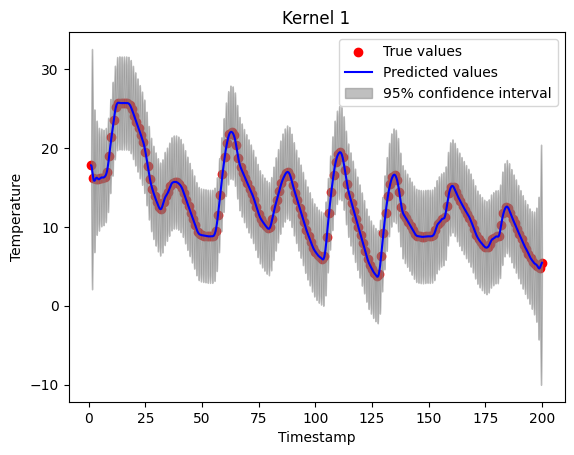
\includegraphics[width=0.8\textwidth]{img/kernel1.png}
\end{center}

\begin{center}
    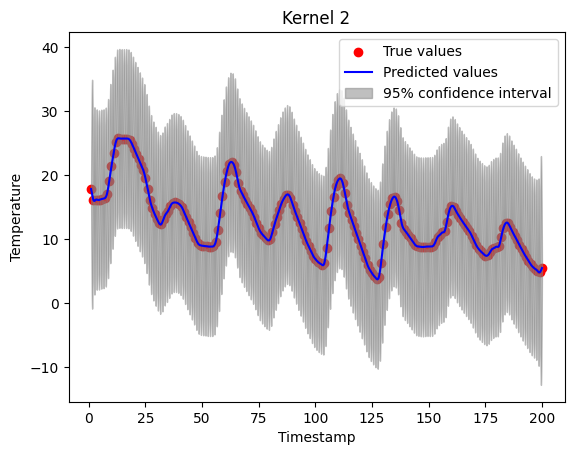
\includegraphics[width=0.8\textwidth]{img/kernel2.png}
\end{center}

\begin{center}
    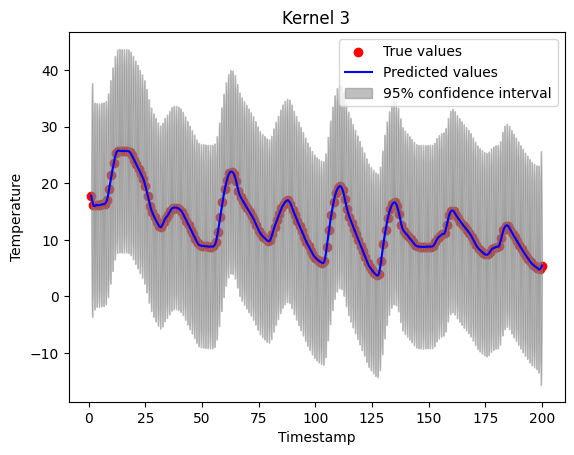
\includegraphics[width=0.8\textwidth]{img/kernel3.png}
\end{center}

\begin{center}
    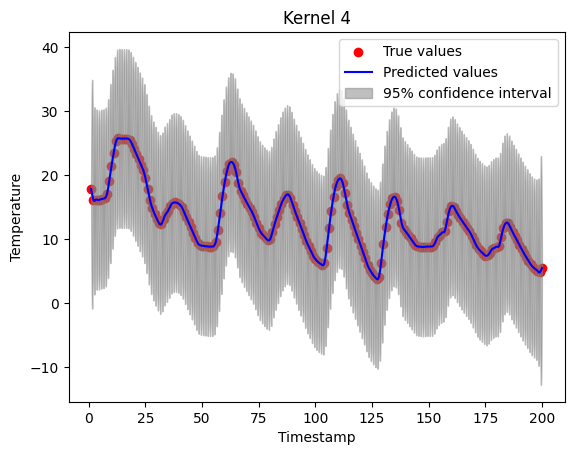
\includegraphics[width=0.8\textwidth]{img/kernel4.png}
\end{center}

\end{document}
